\documentclass{standalone}
\usepackage{tikz}
\usetikzlibrary{patterns, positioning}
\usepackage[sfdefault]{ClearSans} %% option 'sfdefault' activates Clear Sans as the default text font
\usepackage[T1]{fontenc}

\begin{document}
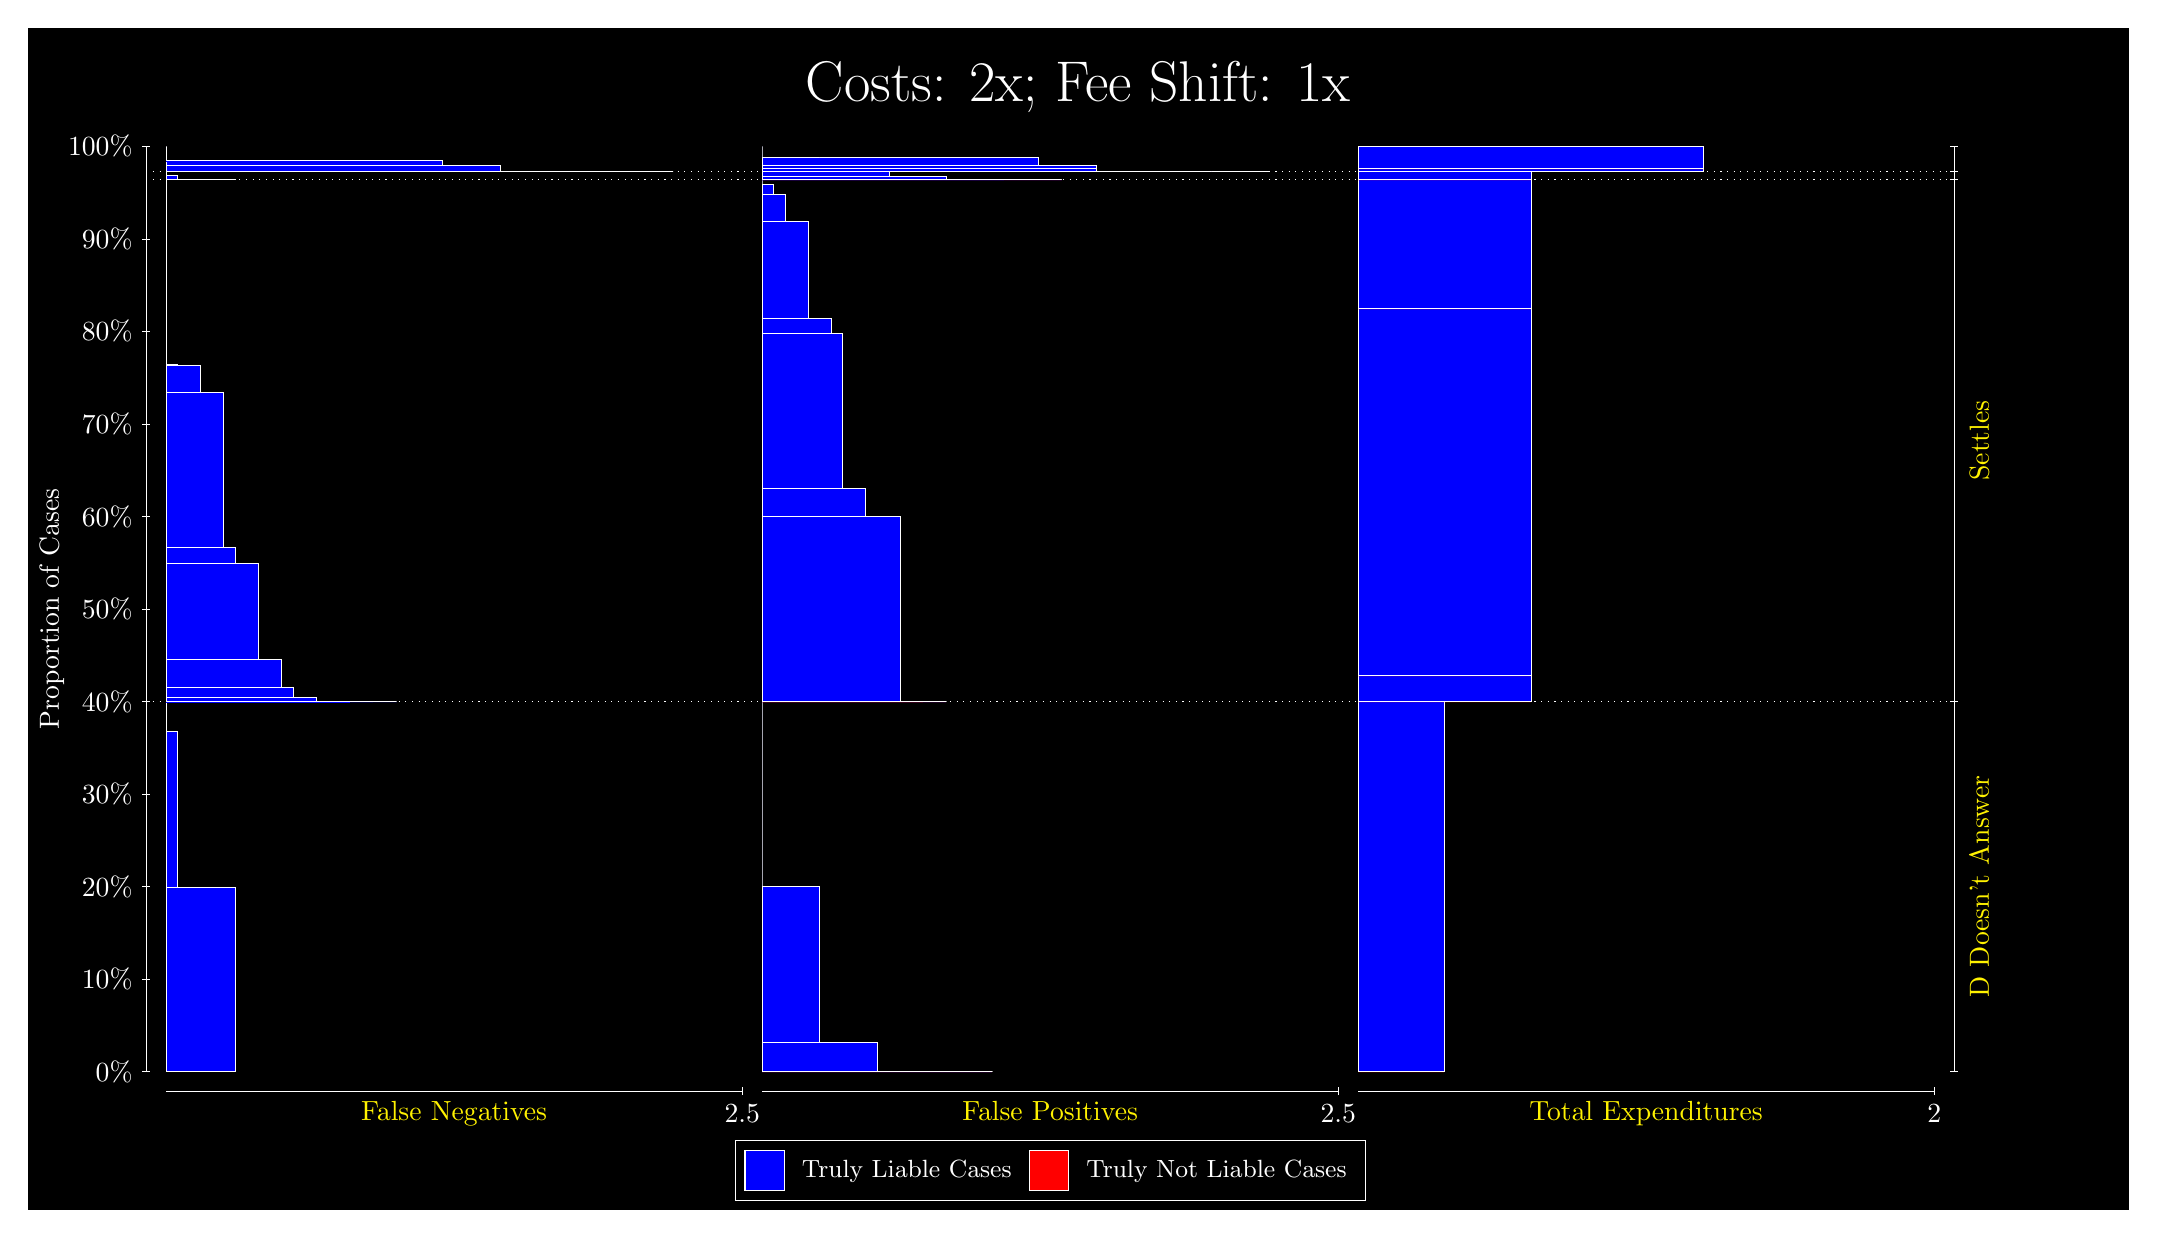
\begin{tikzpicture}
\draw[fill=black] (0,0) rectangle (26.667,15);
\draw[text=white] (0,13.5) rectangle (26.667,15) node[midway] {\huge Costs: 2x; Fee Shift: 1x};
\draw[white, very thin] (1.5,1.75) -- (1.5,13.5);
\node[rotate=90, text=white, anchor=center] at (0.3, 7.625) {Proportion of Cases};
\draw[white, very thin] (1.45,1.75) -- (1.55,1.75);
\node[text=white, anchor=east] at (1.45, 1.75) {0\%};
\draw[white, very thin] (1.45,2.925) -- (1.55,2.925);
\node[text=white, anchor=east] at (1.45, 2.925) {10\%};
\draw[white, very thin] (1.45,4.1) -- (1.55,4.1);
\node[text=white, anchor=east] at (1.45, 4.1) {20\%};
\draw[white, very thin] (1.45,5.275) -- (1.55,5.275);
\node[text=white, anchor=east] at (1.45, 5.275) {30\%};
\draw[white, very thin] (1.45,6.45) -- (1.55,6.45);
\node[text=white, anchor=east] at (1.45, 6.45) {40\%};
\draw[white, very thin] (1.45,7.625) -- (1.55,7.625);
\node[text=white, anchor=east] at (1.45, 7.625) {50\%};
\draw[white, very thin] (1.45,8.8) -- (1.55,8.8);
\node[text=white, anchor=east] at (1.45, 8.8) {60\%};
\draw[white, very thin] (1.45,9.975) -- (1.55,9.975);
\node[text=white, anchor=east] at (1.45, 9.975) {70\%};
\draw[white, very thin] (1.45,11.15) -- (1.55,11.15);
\node[text=white, anchor=east] at (1.45, 11.15) {80\%};
\draw[white, very thin] (1.45,12.325) -- (1.55,12.325);
\node[text=white, anchor=east] at (1.45, 12.325) {90\%};
\draw[white, very thin] (1.45,13.5) -- (1.55,13.5);
\node[text=white, anchor=east] at (1.45, 13.5) {100\%};

\draw[white, very thin] (24.457,1.75) -- (24.457,13.5);
\draw[white, very thin] (24.407,1.75) -- (24.507,1.75);
\node[anchor=west] at (24.407, 1.75) {};
\draw[white, very thin] (24.407,6.4489) -- (24.507,6.4489);
\node[anchor=west] at (24.407, 6.4489) {};
\draw[white, very thin] (24.407,13.078) -- (24.507,13.078);
\node[anchor=west] at (24.407, 13.078) {};
\draw[white, very thin] (24.407,13.182) -- (24.507,13.182);
\node[anchor=west] at (24.407, 13.182) {};
\draw[white, very thin] (24.407,13.5) -- (24.507,13.5);
\node[anchor=west] at (24.407, 13.5) {};

\draw[white, very thin, fill=blue] (1.75,1.75) rectangle (2.6283,4.0962);
\draw[white, very thin, fill=blue] (1.75,4.0962) rectangle (1.8964,6.0728);
\draw[white, very thin, fill=red] (1.75,6.0728) rectangle (1.75,6.0728);
\draw[white, very thin, fill=blue] (1.75,6.0728) rectangle (1.75,6.4489);
\draw[white, very thin, fill=blue] (1.75,6.4489) rectangle (4.6775,6.4489);
\draw[white, very thin, fill=blue] (1.75,6.4489) rectangle (4.3848,6.4489);
\draw[white, very thin, fill=blue] (1.75,6.4489) rectangle (4.092,6.4492);
\draw[white, very thin, fill=blue] (1.75,6.4492) rectangle (3.9457,6.4518);
\draw[white, very thin, fill=blue] (1.75,6.4518) rectangle (3.6529,6.5048);
\draw[white, very thin, fill=blue] (1.75,6.5048) rectangle (3.3602,6.6345);
\draw[white, very thin, fill=blue] (1.75,6.6345) rectangle (3.2138,6.9809);
\draw[white, very thin, fill=blue] (1.75,6.9809) rectangle (2.921,8.211);
\draw[white, very thin, fill=blue] (1.75,8.211) rectangle (2.6283,8.4047);
\draw[white, very thin, fill=blue] (1.75,8.4047) rectangle (2.4819,10.373);
\draw[white, very thin, fill=blue] (1.75,10.373) rectangle (2.1891,10.725);
\draw[white, very thin, fill=blue] (1.75,10.725) rectangle (1.8964,10.728);
\draw[white, very thin, fill=red] (1.75,10.728) rectangle (1.75,10.728);
\draw[white, very thin, fill=blue] (1.75,10.728) rectangle (1.75,13.078);
\draw[white, very thin, fill=blue] (1.75,13.078) rectangle (2.6283,13.079);
\draw[white, very thin, fill=blue] (1.75,13.079) rectangle (1.8964,13.138);
\draw[white, very thin, fill=red] (1.75,13.138) rectangle (1.75,13.138);
\draw[white, very thin, fill=blue] (1.75,13.138) rectangle (1.75,13.182);
\draw[white, very thin, fill=blue] (1.75,13.182) rectangle (8.1906,13.182);
\draw[white, very thin, fill=blue] (1.75,13.182) rectangle (7.4587,13.183);
\draw[white, very thin, fill=blue] (1.75,13.183) rectangle (6.7268,13.189);
\draw[white, very thin, fill=blue] (1.75,13.189) rectangle (5.9949,13.262);
\draw[white, very thin, fill=blue] (1.75,13.262) rectangle (5.2631,13.317);
\draw[white, very thin, fill=blue] (1.75,13.317) rectangle (4.5312,13.317);
\draw[white, very thin, fill=blue] (1.75,13.317) rectangle (3.7993,13.317);
\draw[white, very thin, fill=blue] (1.75,13.317) rectangle (3.2138,13.317);
\draw[white, very thin, fill=blue] (1.75,13.317) rectangle (2.4819,13.318);
\draw[white, very thin, fill=red] (1.75,13.318) rectangle (1.75,13.318);
\draw[white, very thin, fill=blue] (1.75,13.318) rectangle (1.75,13.5);
\draw[white, very thin, fill=red] (9.3189,1.75) rectangle (12.246,1.75);
\draw[white, very thin, fill=blue] (9.3189,1.75) rectangle (12.246,1.75);
\draw[white, very thin, fill=blue] (9.3189,1.75) rectangle (11.515,1.7532);
\draw[white, very thin, fill=blue] (9.3189,1.7532) rectangle (10.783,2.126);
\draw[white, very thin, fill=blue] (9.3189,2.126) rectangle (10.051,4.1027);
\draw[white, very thin, fill=blue] (9.3189,4.1027) rectangle (9.3189,6.4489);
\draw[white, very thin, fill=red] (9.3189,6.4489) rectangle (11.661,6.4489);
\draw[white, very thin, fill=blue] (9.3189,6.4489) rectangle (11.661,6.4489);
\draw[white, very thin, fill=red] (9.3189,6.4489) rectangle (11.368,6.4489);
\draw[white, very thin, fill=blue] (9.3189,6.4489) rectangle (11.368,6.4525);
\draw[white, very thin, fill=red] (9.3189,6.4525) rectangle (11.075,6.4525);
\draw[white, very thin, fill=blue] (9.3189,6.4525) rectangle (11.075,8.7986);
\draw[white, very thin, fill=blue] (9.3189,8.7986) rectangle (10.929,8.8025);
\draw[white, very thin, fill=blue] (9.3189,8.8025) rectangle (10.636,9.1544);
\draw[white, very thin, fill=blue] (9.3189,9.1544) rectangle (10.344,11.122);
\draw[white, very thin, fill=blue] (9.3189,11.122) rectangle (10.197,11.316);
\draw[white, very thin, fill=blue] (9.3189,11.316) rectangle (9.9044,12.546);
\draw[white, very thin, fill=blue] (9.3189,12.546) rectangle (9.6116,12.893);
\draw[white, very thin, fill=blue] (9.3189,12.893) rectangle (9.4652,13.022);
\draw[white, very thin, fill=blue] (9.3189,13.022) rectangle (9.3189,13.078);
\draw[white, very thin, fill=red] (9.3189,13.078) rectangle (13.125,13.078);
\draw[white, very thin, fill=blue] (9.3189,13.078) rectangle (13.125,13.078);
\draw[white, very thin, fill=blue] (9.3189,13.078) rectangle (12.393,13.078);
\draw[white, very thin, fill=blue] (9.3189,13.078) rectangle (11.661,13.123);
\draw[white, very thin, fill=blue] (9.3189,13.123) rectangle (10.929,13.181);
\draw[white, very thin, fill=blue] (9.3189,13.181) rectangle (10.197,13.182);
\draw[white, very thin, fill=red] (9.3189,13.182) rectangle (15.759,13.182);
\draw[white, very thin, fill=blue] (9.3189,13.182) rectangle (15.759,13.182);
\draw[white, very thin, fill=blue] (9.3189,13.182) rectangle (15.028,13.182);
\draw[white, very thin, fill=red] (9.3189,13.182) rectangle (15.028,13.182);
\draw[white, very thin, fill=blue] (9.3189,13.182) rectangle (15.028,13.182);
\draw[white, very thin, fill=blue] (9.3189,13.182) rectangle (14.296,13.186);
\draw[white, very thin, fill=red] (9.3189,13.186) rectangle (14.296,13.186);
\draw[white, very thin, fill=blue] (9.3189,13.186) rectangle (14.296,13.187);
\draw[white, very thin, fill=blue] (9.3189,13.187) rectangle (13.564,13.217);
\draw[white, very thin, fill=blue] (9.3189,13.217) rectangle (13.564,13.26);
\draw[white, very thin, fill=blue] (9.3189,13.26) rectangle (12.832,13.261);
\draw[white, very thin, fill=blue] (9.3189,13.261) rectangle (12.832,13.364);
\draw[white, very thin, fill=blue] (9.3189,13.364) rectangle (12.1,13.366);
\draw[white, very thin, fill=blue] (9.3189,13.366) rectangle (11.368,13.366);
\draw[white, very thin, fill=red] (9.3189,13.366) rectangle (10.783,13.366);
\draw[white, very thin, fill=blue] (9.3189,13.366) rectangle (10.783,13.366);
\draw[white, very thin, fill=red] (9.3189,13.366) rectangle (10.051,13.366);
\draw[white, very thin, fill=blue] (9.3189,13.366) rectangle (10.051,13.366);
\draw[white, very thin, fill=red] (9.3189,13.366) rectangle (9.3189,13.366);
\draw[white, very thin, fill=blue] (9.3189,13.366) rectangle (9.3189,13.5);
\draw[white, very thin, fill=red] (16.888,1.75) rectangle (17.986,1.75);
\draw[white, very thin, fill=blue] (16.888,1.75) rectangle (17.986,6.4489);
\draw[white, very thin, fill=red] (16.888,6.4489) rectangle (19.083,6.4489);
\draw[white, very thin, fill=blue] (16.888,6.4489) rectangle (19.083,6.7766);
\draw[white, very thin, fill=red] (16.888,6.7766) rectangle (19.083,6.7766);
\draw[white, very thin, fill=blue] (16.888,6.7766) rectangle (19.083,11.44);
\draw[white, very thin, fill=red] (16.888,11.44) rectangle (19.083,11.44);
\draw[white, very thin, fill=blue] (16.888,11.44) rectangle (19.083,13.078);
\draw[white, very thin, fill=red] (16.888,13.078) rectangle (19.083,13.078);
\draw[white, very thin, fill=blue] (16.888,13.078) rectangle (19.083,13.182);
\draw[white, very thin, fill=red] (16.888,13.182) rectangle (21.279,13.182);
\draw[white, very thin, fill=blue] (16.888,13.182) rectangle (21.279,13.218);
\draw[white, very thin, fill=red] (16.888,13.218) rectangle (21.279,13.218);
\draw[white, very thin, fill=blue] (16.888,13.218) rectangle (21.279,13.5);
\draw[white, dotted] (1.5,6.4489) -- (24.457,6.4489);
\draw[white, dotted] (1.5,13.078) -- (24.457,13.078);
\draw[white, dotted] (1.5,13.182) -- (24.457,13.182);
\draw[white, very thin] (1.75,1.5) -- (9.0689,1.5);
\node[text=yellow, anchor=north] at (5.4094, 1.5) {False Negatives};
\draw[white, very thin] (9.0689,1.45) -- (9.0689,1.55);
\node[text=white, anchor=north] at (9.0689, 1.45) {2.5};

\draw[white, very thin] (9.3189,1.5) -- (16.638,1.5);
\node[text=yellow, anchor=north] at (12.978, 1.5) {False Positives};
\draw[white, very thin] (16.638,1.45) -- (16.638,1.55);
\node[text=white, anchor=north] at (16.638, 1.45) {2.5};

\draw[white, very thin] (16.888,1.5) -- (24.207,1.5);
\node[text=yellow, anchor=north] at (20.547, 1.5) {Total Expenditures};
\draw[white, very thin] (24.207,1.45) -- (24.207,1.55);
\node[text=white, anchor=north] at (24.207, 1.45) {2};

\node[text=yellow, centered, rotate=90] at (24.777, 4.0994) {D Doesn't Answer};
\node[text=yellow, centered, rotate=90] at (24.777, 9.7635) {Settles};



\draw (12.978300999999998,1.5) node[draw=none] (baseCoordinate) {};
\begin{scope}[align=center]
        \matrix[scale=0.5, draw=white, below=0.5cm of baseCoordinate, nodes={draw}, column sep=0.1cm]{
            \node[rectangle, draw, minimum width=0.5cm, minimum height=0.5cm, fill=blue] {}; &
            \node[draw=none, font=\small, text=white] (B) {Truly Liable Cases}; &
            \node[rectangle, draw, minimum width=0.5cm, minimum height=0.5cm, fill=red] {}; &
            \node[draw=none, font=\small, text=white] (B) {Truly Not Liable Cases}; \\
            };
\end{scope}

\end{tikzpicture}
\end{document}